\section{The Road-network Model}

The road-network used for fisse experimentation is extracted
from Open Street Maps (OSM) and converted into a more suitable 
graph representation. Our graph representation consists 
of edges which represents roads and vertices which represents 
either charge stations or road intersections. A road is 
a double of distance (km), $d$, and speed limit (km/h), 
$V_{lim}$:

\[E(V_i, V_j) = \{d, V_{lim}\} \]

Where $V_i$ and $V_j$ are adjacent vertices. A vertex is a 
single of charge rate (kWh/h), $R_{charge}$:

\[V = \{R_{charge}\} \]

A road intersection is simply a vertex with $R_{charge} = 0$
while a charge station is a vertex where $R_{charge} > 0$. 
An electrical vehicle is specified by two parameters: It's 
battery capacity (kWh), consumption rate (kWh/km). The 
consumption rate is given by the following function:

\[ 4,60272*10^{-5}*v^2+6,59187*10^{-4}*v+0,173117 \]

where $v$ is the speed of the vehicle. 

\begin{figure}
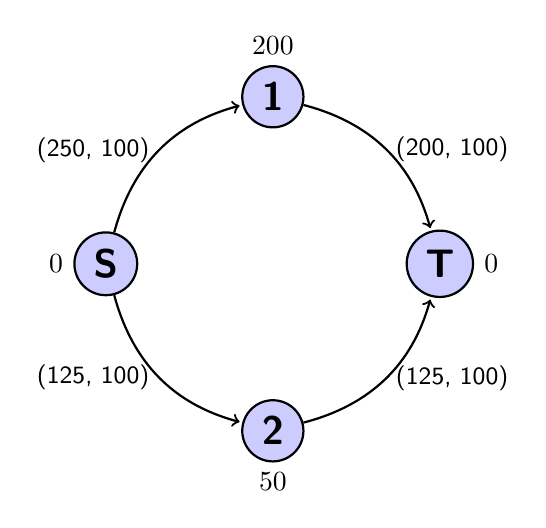
\begin{tikzpicture}[->,->,shorten >=1pt,auto,node distance=3cm,
  thick,main node/.style={circle,fill=blue!20,draw,font=\sffamily\Large\bfseries}]
%1
  \node[main node] (1) {1};
  \node[above] at (1.north) {200};
%2 
 \node[main node] (2) [below left of=1] {S};
  \node[left] at (2.west) {0};
%3 
 \node[main node] (3) [below right of=2] {2};
  \node[below] at (3.south) {50};
%4 
 \node[main node] (4) [below right of=1] {T};
  \node[right] at (4.east) {0};
%paths
  \path[every node/.style={font=\sffamily\small}]
    (1)
	  edge [bend left] node[right] {(200, 100)} (4)
    (2) edge [bend right] node[left] {(125, 100)} (3)
    	  edge [bend left] node[left] {(250, 100)} (1)
    (3) edge [bend right] node[right] {(125, 100)} (4)
    (4) ;
\end{tikzpicture}
\label{figure:simpleroad-network}
\caption{A simple road-network with starting point s and end point t}
\end{figure}